\documentclass[11pt]{charter}

\usepackage{makecell}
\usepackage{lscape}

% El títulos de la memoria, se usa en la carátula y se puede usar el cualquier lugar del documento con el comando \ttitle
\titulo{Red de sensores inalámbricos en invernaderos automatizados} 

% Nombre del posgrado, se usa en la carátula y se puede usar el cualquier lugar del documento con el comando \degreename
%\posgrado{Carrera de Especialización en Sistemas Embebidos} 
\posgrado{Carrera de Especialización en Sistemas Embebidos} 
%\posgrado{Carrera de Especialización en Intelegencia Artificial}
%\posgrado{Maestría en Sistemas Embebidos} 
%\posgrado{Maestría en Internet de las cosas}

% Tu nombre, se puede usar el cualquier lugar del documento con el comando \authorname
\autor{Ing. Maximiliano Sarli} 

% El nombre del director y co-director, se puede usar el cualquier lugar del documento con el comando \supname y \cosupname y \pertesupname y \pertecosupname
\director{Mg. Ing. Gonzalo Sanchez}
\pertenenciaDirector{FIUBA} 
% FIXME:NO IMPLEMENTADO EL CODIRECTOR ni su pertenencia
\codirector{} % si queda vacio no se deberíá incluir 
\pertenenciaCoDirector{}

% Nombre del cliente, quien va a aprobar los resultados del proyecto, se puede usar con el comando \clientename y \empclientename
\cliente{Pablo Lodetti}
\empresaCliente{Wentux}

% Nombre y pertenencia de los jurados, se pueden usar el cualquier lugar del documento con el comando \jurunoname, \jurdosname y \jurtresname y \perteunoname, \pertedosname y \pertetresname.
\juradoUno{Nombre y Apellido (1)}
\pertenenciaJurUno{pertenencia (1)} 
\juradoDos{Nombre y Apellido (2)}
\pertenenciaJurDos{pertenencia (2)}
\juradoTres{Nombre y Apellido (3)}
\pertenenciaJurTres{pertenencia (3)}
 
\fechaINICIO{25 de agosto de 2020}		%Fecha de inicio de la cursada de GdP \fechaInicioName
\fechaFINALPlanificacion{13 de octubre de 2020} 	%Fecha de final de cursada de GdP
\fechaFINALTrabajo{23 de agosto de 2021}		%Fecha de defensa pública del trabajo final


\begin{document}

\maketitle
\thispagestyle{empty}
\pagebreak


\thispagestyle{empty}
{\setlength{\parskip}{0pt}
\tableofcontents{}
}
\pagebreak


\section{Registros de cambios}
\label{sec:registro}


\begin{table}[ht]
\label{tab:registro}
\centering
\begin{tabularx}{\linewidth}{@{}|c|X|c|@{}}
\hline
\rowcolor[HTML]{C0C0C0} 
Revisión & \multicolumn{1}{c|}{\cellcolor[HTML]{C0C0C0}Detalles de los cambios realizados} & Fecha      \\ \hline
1.0      & Creación del documento                                          & 02/11/2020 \\ \hline
1.1      & Avances hasta definición de requerimientos                                          & 04/11/2020 \\ \hline
1.2      & Cierre primer entregable con WBS terminada
& 06/11/2020 \\ \hline
1.3      & Correciones de la primer entrega e historias de usuarios
& 06/11/2020 \\ \hline
1.4      & Tercer entrega y correcciones detectadas
& 21/11/2020 \\ \hline
1.5      & Tercer entrega últimos puntos y corrección presupuesto
& 22/11/2020 \\ \hline
1.6      & Cuarta entrega
& 28/11/2020 \\ \hline
1.7      & Correcciones segunda y tercer entrega. Cambios propuestos por el cliente
& 29/11/2020 \\ \hline
\end{tabularx}
\end{table}

\pagebreak



\section{Acta de constitución del proyecto}
\label{sec:acta}

\begin{flushright}
Buenos Aires, \fechaInicioName
\end{flushright}

\vspace{2cm}

Por medio de la presente se acuerda con el Ing. \authorname\hspace{1px} que su Trabajo Final de la \degreename\hspace{1px} se titulará ``\ttitle'', consistirá en el desarrollo de un sistema de control inalámbrico y de bajo costo para invernaderos y/o indoors domésticos, y tendrá un presupuesto preliminar estimado de 603 hs de trabajo y {\$6.602}, con fecha de inicio \fechaInicioName\hspace{1px} y fecha de presentación pública \fechaFinalName.

Se adjunta a esta acta la planificación inicial.

\vfill

% Esta parte se construye sola con la información que hayan cargado en el preámbulo del documento y no debe modificarla
\begin{table}[ht]
\centering
\begin{tabular}{ccc}
\begin{tabular}[c]{@{}c@{}}Ariel Lutenberg \\ Director posgrado FIUBA\end{tabular} & \hspace{2cm} & \begin{tabular}[c]{@{}c@{}}\clientename \\ \empclientename \end{tabular} \vspace{2.5cm} \\ 
\multicolumn{3}{c}{\begin{tabular}[c]{@{}c@{}} \supname \\ Director del Trabajo Final\end{tabular}} \vspace{2.5cm} \\
%\begin{tabular}[c]{@{}c@{}}\jurunoname \\ Jurado del Trabajo Final\end{tabular}     &  & \begin{tabular}[c]{@{}c@{}}\jurdosname\\ Jurado del Trabajo Final\end{tabular}  \vspace{2.5cm}  \\
%\multicolumn{3}{c}{\begin{tabular}[c]{@{}c@{}} \jurtresname\\ Jurado del Trabajo Final\end{tabular}} \vspace{.5cm}                                                                     
\end{tabular}
\end{table}




\section{Descripción técnica-conceptual del proyecto a realizar}
\label{sec:descripcion}

\begin{consigna}{black}
La empresa Wentux ha desarrollado un sistema de control para invernaderos y/o indoors domésticos de bajo costo y que requiere mínimo conocimiento técnico y electrónico para su instalación y puesta en funcionamiento. Este sistema, controla y monitorea variables como humedad, temperatura, ventilación, riego, calefacción, co2 e iluminación.
Las distintas variables de control se visualizan mediante un dispositivo móvil o una computadora.

En la actualidad, en el sistema de control, los diversos sensores se conectan a través de cables a un sistema embebido central que procesa la información recibida. La solución actual, atenta contra la comodidad y simpleza de instalación que la empresa tiene como objetivo en sus equipos. Por tal motivo, se tiene como propósito, reemplazar el cableado por una red de sensores inalámbrica (Wireless Sensor Network), por la cual se envíen los datos recolectados de los cultivos al dispositivo embebido central.

Esta solución deberá ser flexible y de fácil adaptación a cualquier tipo de invernadero y/o indoor, así como también, deberá implementar funciones de ahorro de energía para alargar la vida útil de las baterías utilizadas en cada sensor inalámbrico.
Cada sensor inalámbrico (de ahora en más "nodo"), estará compuesto por un conjunto de componentes: microcontrolador, módulo inalámbrico, sensor y batería. Estos nodos, se comunicarán con la central a través de la red inalámbrica, usando un protocolo de comunicación entre ellos, cuya creación y método de encriptado forma parte del desarrollo de la solución.

En la figura \ref{fig:diagBloques} se observa el diagrama de bloques de la solución a abordar. Como se mencionó anteriormente, se pueden observar los distintos nodos de la red de sensores inalámbrica, compuestos por el conjunto de componentes detallado. Estos nodos se comunicarán con otro nodo central que estará embebido en el sistema de control que ya tiene desarrollado Wentux, con el cual deberán comunicarse usando el protocolo de comunicación a desarrollar.

El nodo central no tendrá una batería ni ningún tipo de sensor. Este nodo se utilizará como receptor "maestro" {} que recibirá toda la información obtenida de los distintos nodos, y a su vez, como emisor  "maestro" {} para dar instrucciones a los nodos de su red, o bien, para configurar valores en cada nodo.
Finalmente, el nodo maestro es quien hará disponible la información recavada de los nodos en el dispositivo móvil o computadora.

\vspace{25px}

\begin{figure}[htpb]
\centering 
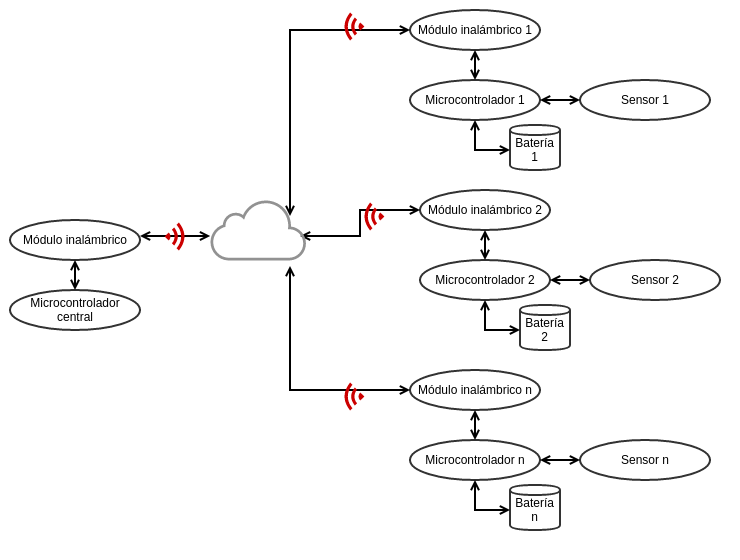
\includegraphics[width=.9\textwidth]{./Figuras/Figura1.png}
\caption{Diagrama en bloques del sistema}
\label{fig:diagBloques}
\end{figure}

\vspace{25px}

\end{consigna}




\section{Identificación y análisis de los interesados}
\label{sec:interesados}

\begin{consigna}{black} 

\begin{table}[ht]
%\caption{Identificación de los interesados}
%\label{tab:interesados}
\begin{tabularx}{\linewidth}{@{}|l|X|X|l|@{}}
\hline
\rowcolor[HTML]{C0C0C0} 
Rol           & Nombre y Apellido & Organización 	& Puesto 	\\ \hline
Cliente       & \clientename      &\empclientename	& Director Wentux       \\ \hline
Responsable   & \authorname       & FIUBA        	& Alumno 	\\ \hline
Colaboradores & Raúl Palavecino   & -             	& Estudiante ingeniería electrónica       	\\ \hline
Orientador    & \supname	      & \pertesupname 	& Director	Trabajo final \\ \hline
Usuario final & Productores e \newline independientes \newline pequeña/mediana \newline escala. \newline Agricultura, \newline frutihortícola, plantas \newline ornamentales. Profesionales \newline dedicados a \newline climatizar \newline recintos para \newline diversos usos.                 & -             	& -       	\\ \hline
\end{tabularx}
\end{table}


\begin{itemize}
\item Cliente Pablo Lodeti: Director de Wentux. Desarrolló el actual producto que tiene la empresa.
\item Colaborador Raúl Palavecino: estudiante de la carrera ingeniería en electrónica y persona con experiencia en embebidos. 
\item Orientador Gonzalo Sanchez: magister en sistema embebidos con experiencia en el microcontrolador a utilizar.
\end{itemize}

\end{consigna}



\section{1. Propósito del proyecto}
\label{sec:proposito}

\begin{consigna}{black}

El propósito del proyecto es desarrollar una red de sensores inalámbrica para eliminar las incomodidades y restricciones que genera el cableado actual que tienen los equipos. De esta forma, la nueva red de sensores inalámbrica beneficiará la instalación y la comodidad en el uso diario de los equipos.
\end{consigna}

\section{2. Alcance del proyecto}
\label{sec:alcance}

\begin{consigna}{black}
El proyecto incluye el desarrollo del firmware para la comunicación de los nodos con la central, prueba de prototipo  funcional y su puesta en funcionamiento en una pequeña  planta  dentro de las instalaciones del  taller o en  planta modelo  montada por colaborador  para pruebas, que simule el  invernadero a controlar. También se incluye el desarrollo del hardware del conjunto microcontrolador, sensor, batería y módulo inalámbrico (nodos). 

El proyecto no incluye la puesta en funcionamiento en campo y posterior mantenimiento .

\end{consigna}


\section{3. Supuestos del proyecto}
\label{sec:supuestos}

\begin{consigna}{black}

\begin{itemize}
\item El cliente proveerá los fondos para la compra de sensores,  actuadores y materiales varios para desarrollar la red de sensores.
\item El cliente deberá proveer un equipo funcionando con el cual la red de sensores deberá comunicarse.
\item El cliente proveerá un entorno o invernadero/indoor piloto de prueba.
\end{itemize}

\end{consigna}

\section{4. Requerimientos}
\label{sec:requerimientos}

\begin{consigna}{black}
Los requerimientos surgen del análisis realizado a la propuesta y del relevamiento del proyecto que envía el cliente. Estos se detallan a continuación, agrupados por afinidad y se indica en cada uno su prioridad, siendo [0] la más alta y [3] la más baja.

\begin{enumerate}
\item Grupo de requerimientos asociados con comunicación
	\begin{enumerate}
	\item Cada nodo deberá enviar la información tomada del sensor a la central. El período de muestreo deberá ser configurable desde la central. Cada mensaje hacia la central tendrá un máximo de 10 bytes [0].
	\item Se deberá desarrollar un protocolo de comunicación entre la central y los nodos [0].
	\item Los nodos tendrán un sistema de reintento de envío de información a la central en caso de falla [2].
	\item Los nodos almacenarán en memoria interna información no enviada hasta que se envíe en un reintento [3].
	\item La comunicación deberá estar protegida mediante un algoritmo de encriptación para que no sea alterada externamente [3].
	\end{enumerate}
\item Grupo de requerimientos asociados con alimentación
	\begin{enumerate}
	\item Los nodos estarán alimentados por batería como fuente eléctrica, el rango de tensión admisible será de 1,9 v a 3,3 v. La tensión nominal será de 3,3 v. La batería deberá durar 30 días como mínimo [0].
	\item Se deberá desarrollar una función de ahorro de batería en los nodos [1].
	\end{enumerate}
\item Grupo de requerimientos asociados con generalidades del proyecto
	\begin{enumerate}
	\item Cada nodo estará compuesto por un conjunto de microcontrolador, módulo inalámbrico, sensor y batería. El sistema tendrá un máximo de seis sensores y la distancia máxima a la central será de 15 metros [0].
	\item El sistema debe permitir instalarse en cualquier invernadero o indoor [2].
	\end{enumerate}
\item Grupo de requerimientos asociados con documentación y codificación
	\begin{enumerate}
	\item Se deberá entregar un manual de instalación y manual de uso [3].
	\item Se deberá usar Git como software de control de versiones [2].
	\item Se deberá documentar el código con doxygen [3].
	\end{enumerate}


\end{enumerate}

\end{consigna}

\section{Historias de usuarios (\textit{Product backlog})}
\label{sec:backlog}

\begin{consigna}{black}

Se enumeran las historias de usuario y su ponderación calculada en story points (del [1] al [5]).

\begin{enumerate}
\item Como productor de invernadero del producto quiero poder visualizar la información obtenida de los sensores en tiempo real para tener un mejor control de las variables controladas [2].

\item Como productor de invernadero del producto quiero configurar los tiempos de sensado de cada nodo para darle un tratado diferencial a cada plantación de mis cultivos [2].

\item Como productor doméstico del producto quiero instalarlo de manera práctica, flexible y sin conocimiento técnico para no tener que involucrarme en cuestiones técnicas del producto [1].

\item Como cliente del proyecto quiero eliminar el cableado del producto final para ofrecer un producto con mayor estética visual y practicidad en su uso [5].

\item Como cliente del proyecto quiero despreocuparme de la duración de las baterías para que el producto requiera mínimo control de funcionamiento [4].

\item Como cliente del proyecto quiero utilizar un microcontrolador STM 32 para abaratar los costos del producto [4].

\end{enumerate}


\end{consigna}

\section{5. Entregables principales del proyecto}
\label{sec:entregables}

\begin{consigna}{black}
Los entregables del proyecto son:

\begin{itemize}
\item Informe de avance
\item Manual de uso
\item Código fuente
\item Prototipo funcional
\item Manual de instalación
\item Memoria técnica

\end{itemize}

\end{consigna}

\section{6. Desglose del trabajo en tareas}
\label{sec:wbs}

\begin{consigna}{black}
El proyecto se divide en las siguientes tareas:

\begin{enumerate}
\item \textbf{Gestión del proyecto: 68 hs}
	\begin{enumerate}
	\item Planificación del proyecto (20 hs)
	\item Confección informe de avance (8 hs)
	\item Análisis y relevamiento inicial (15 hs)
	\item Confección manual de instalación (10 hs)
	\item Confección manual de uso (15 hs)
	\end{enumerate}
\item \textbf{Hardware: 42 hs}
	\begin{enumerate}
	\item Definición de componentes (7 hs)
	\item Compra de componentes (5 hs)
	\item Diseño de prototipos de los nodos (10 hs)
	\item Elaboración/construcción de los nodos (20 hs)
	\end{enumerate}
\item \textbf{Firmware: 238 hs}
	\begin{enumerate}
	\item Diseño de la solución (28 hs)
	\item Configuración de herramientas y plataforma de desarrollo (21 hs)
	\item Estudio y aprendizaje para el desarrollo de los componentes (20 hs)
	\item Desarrollo del protocolo de comunicación y su encriptación (40 hs)
	\item Desarrollo de la función ahorro de batería (33 hs)
	\item Desarrollo de configuración inicial de nuevo nodo en la red (35 hs)
	\item Desarrollo de los componentes de medición y almacenamiento (32 hs)
	\item Desarrollo del módulo de reenvío (29 hs)
	\end{enumerate}
\item \textbf{Testing y verificación: 115 hs}
	\begin{enumerate}
	\item Testing unitario del protocolo de comunicación (20 hs)
	\item Testing unitario de la función de ahorro de batería (15 hs)
	\item Testing unitario de nuevo nodo en red (18 hs)
	\item Testing unitario de la medición, almacenamiento y reenvío (25 hs)
	\item Testing de integración (37 hs)
	\end{enumerate}
\item \textbf{Implementación e integración: 50 hs}
	\begin{enumerate}
	\item Integración de los componentes con un producto final (20 hs)
	\item Implementación del prototipo en una planta real (indoor o invernadero) (30 hs)
	\end{enumerate}
\item \textbf{Presentación del trabajo: 90 hs}
	\begin{enumerate}
	\item Confección de la memoria (70 hs)
	\item Preparación de la presentación final (20 hs)
	\end{enumerate}
\end{enumerate}

\textbf{Cantidad total de horas: (603 hs)}


\end{consigna}

\section{7. Diagrama de Activity On Node}
\label{sec:AoN}

\begin{consigna}{black}

En la figura \ref{fig:aon} se detalla el diagrama de \textbf{\textit{Activity On Node}} {} asociado a las tareas del proyecto. Los colores representan las agrupaciones que se realizaron en el desglose del trabajo en tareas, estas son:

\begin{enumerate}
	\item Gestión del proyecto (celeste)
	\item Hardware (lila)
	\item Firmware (colorado)
	\item Testing y verificación (amarillo)
	\item Implementación e integración (verde)
	\item Presentación del trabajo (gris)
\end{enumerate}

%La figura \ref{fig:AoN} fue elaborada con el paquete latex tikz y pueden consultar la siguiente referencia \textit{online}:

%\url{https://www.overleaf.com/learn/latex/LaTeX_Graphics_using_TikZ:_A_Tutorial_for_Beginners_(Part_3)\%E2\%80\%94Creating_Flowcharts}

\end{consigna}

\begin{figure}[htpb]
\centering 
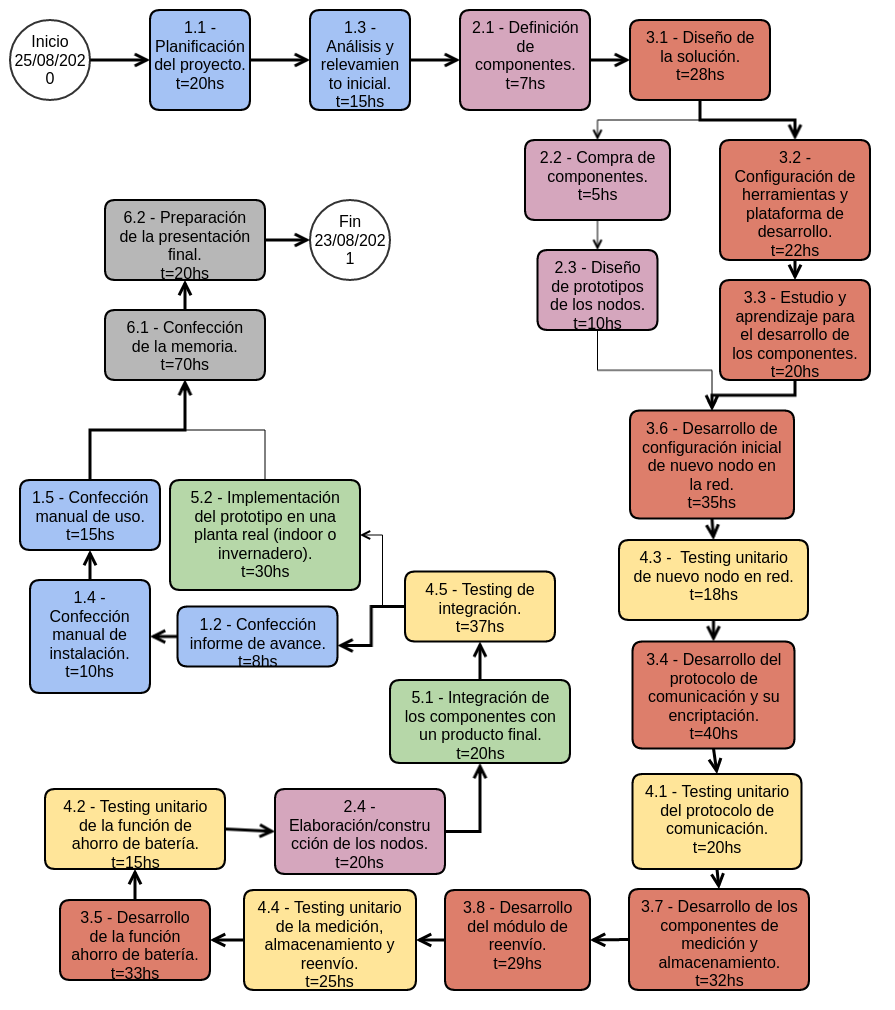
\includegraphics[width=16cm]{./Figuras/aon.png}
\caption{Diagrama en \textit{Activity on Node}}
\label{fig:aon}
\end{figure}


\section{8. Diagrama de Gantt}
\label{sec:gantt}

\begin{consigna}{black}

En la figura \ref{fig:wbs} se detalla la tabla asociada al diagrama de Gantt. En la figura \ref{fig:g1} se detalla el diagrama de Gantt asociado a las tareas y sus fechas correspondientes.

\begin{figure}[htpb]
\centering 
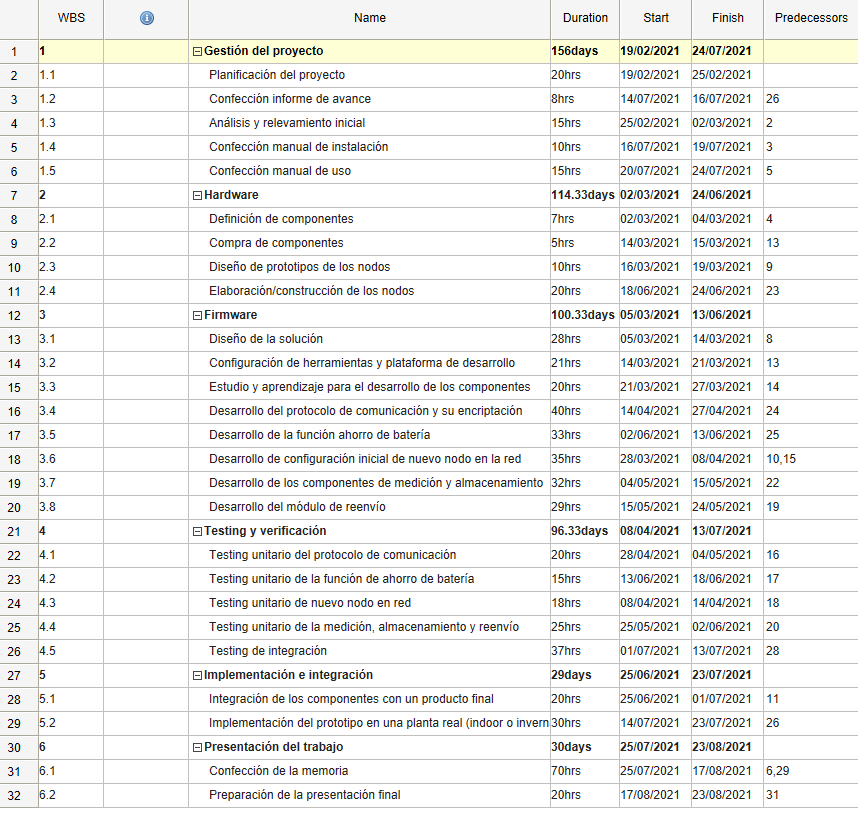
\includegraphics[width=18cm]{./Figuras/wbs.png}
\caption{Tabla diagrama de Gantt}
\label{fig:wbs}
\end{figure}

\begin{landscape}
\begin{figure}[htpb]
\centering 
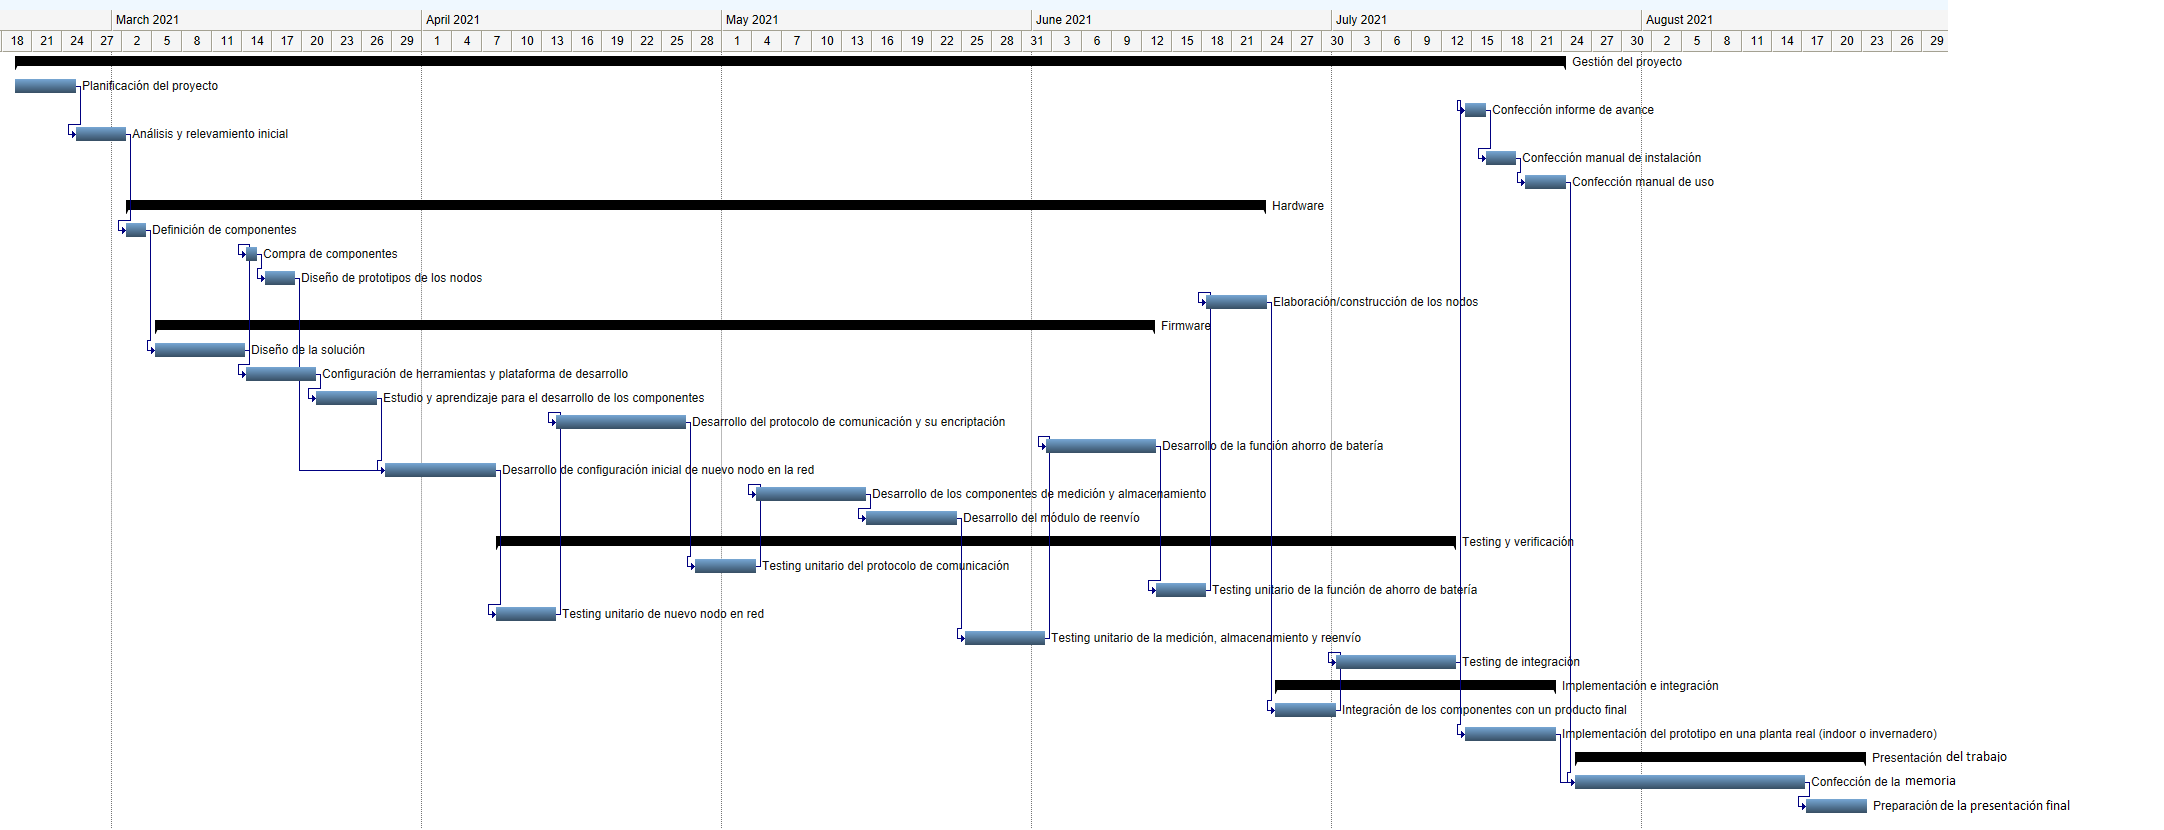
\includegraphics[width=25cm,height=13cm]{./Figuras/calendar.png}
\caption{Diagrama de Gantt}
\label{fig:g1}
\end{figure}
\end{landscape}

\end{consigna}

\section{9. Matriz de uso de recursos de materiales}
\label{sec:recursos}

Para la ejecución del proyecto se precisan los siguientes materiales:

\begin{enumerate}
	\item Microcontrolador Blue Pill Stm32f103c8t6 (x4 unidades)
	\item Módulo transceptor Rf Nrf24l01 2,4 GHz Arduino pic avr (x4 unidades)
	\item Sensor de humedad y temperatura Htu2 (x3 unidades)
	\item PC (x1 unidad)
	\item Planta real (indoor o invernadero)
	\item Producto actual cableado
	\item Pila D (x6 unidades)
\end{enumerate}



\begin{table}
\label{tab:recursos}
\centering
\begin{tabularx}{\linewidth}{@{}|X|c|X|X|X|X|X|X|X|@{}}
\hline
\cellcolor[HTML]{C0C0C0} & \cellcolor[HTML]{C0C0C0} & \multicolumn{7}{c|}{\cellcolor[HTML]{C0C0C0}Recursos requeridos (horas)} \\ \cline{3-9} 
\multirow{-2}{*}{\cellcolor[HTML]{C0C0C0}\begin{tabular}[c]{@{}c@{}}Código\\ WBS\end{tabular}} & \multirow{-2}{*}{\cellcolor[HTML]{C0C0C0}\begin{tabular}[c]{@{}c@{}}Nombre \\ tarea\end{tabular}} & Micro & NRF & Sensor & PC & Planta & Prod & Pila \\ \hline

1.1 & \makecell{Planificación \\ del proyecto}  &  &  &  & 20 & & &\\ \hline
1.2 & \makecell{Confección informe \\ de avance} &  &  &  & 8 & & &  \\ \hline
1.3 & \makecell{Análisis y relevamiento \\ inicial} &  &  &  & 15 & & & \\ \hline
1.4 & \makecell{Confección manual \\ de instalación} &  &  &  & 8 & & 2 & \\ \hline
1.5 & \makecell{Confección manual \\ de uso} &  &  &  & 13 & & 2 & \\ \hline
2.1 & \makecell{Definición de \\ componentes} &  &  &  &  7 & & & \\ \hline
2.2 & \makecell{Compra de \\componentes} &  &  &  & 5 & & & \\ \hline
2.3 & \makecell{Diseño de prototipos \\ de los nodos} &  &  &  & 10 & & & \\ \hline 
2.4 & \makecell{Elaboración/construcción \\ de los nodos} & 20 & 20 & 15 &  & & &\\ \hline
3.1 & Diseño de la solución &  &  &  & 28 & &  &\\ \hline
3.2 & \makecell{Configuración de  \\ herramientas y  \\ plataforma de\\ desarrollo}  & 10 &  &  & 21 & & &\\ \hline

3.3 & \makecell{Estudio y aprendizaje \\ para el desarrollo  \\ de los componentes} & 20 &  &  & 20 & &  &\\ \hline
3.4 & \makecell{Desarrollo del \\ protocolo de \\ comunicación y su\\ encriptación} & 40 & 40 &  & 40 & &  &\\ \hline
3.5 & \makecell{Desarrollo de la \\ función ahorro de \\ batería} & 33 &  33 &  & 33 & & & 30 \\ \hline
3.6 & \makecell{Desarrollo de \\configuración inicial\\ de nuevo nodo \\ en la red} & 35 & 35 &  & 35 & &  & \\ \hline
3.7 & \makecell{Desarrollo de los \\ componentes de \\  medición y \\ almacenamiento} & 32 & 32 & 32 & 32 & & & \\ \hline

\end{tabularx}%
\end{table}


\begin{table}
\label{tab:recursos}
\centering
\begin{tabularx}{\linewidth}{@{}|X|c|X|X|X|X|X|X|X|@{}}
\hline
\cellcolor[HTML]{C0C0C0} & \cellcolor[HTML]{C0C0C0} & \multicolumn{7}{c|}{\cellcolor[HTML]{C0C0C0}Recursos requeridos (horas)} \\ \cline{3-9} 
\multirow{-2}{*}{\cellcolor[HTML]{C0C0C0}\begin{tabular}[c]{@{}c@{}}Código\\ WBS\end{tabular}} & \multirow{-2}{*}{\cellcolor[HTML]{C0C0C0}\begin{tabular}[c]{@{}c@{}}Nombre \\ tarea\end{tabular}} & 1.Micro & 2.NRF & 3.Sensor & 4.PC & 5.Planta & 6.Prod & 7.Pila \\ \hline


3.8 & \makecell{Desarrollo del \\ módulo de reenvío} & 29 & 29 &  & 29 & & & \\ \hline
4.1 & \makecell{Testing unitario \\del protocolo de \\comunicación} & 20 & 20 &  & 20 & & & \\ \hline

4.2 & \makecell{Testing unitario de \\ la función de ahorro\\ de batería} & 15 & 15 &  & 15 & & & 15 \\ \hline
4.3 & \makecell{Testing unitario de \\ nuevo nodo en red} & 18 & 18 &  & 18 & & & \\ \hline
4.4 & \makecell{Testing unitario de \\la medición, \\almacenamiento y\\ reenvío} & 25 & 25 & 25 & 25 & & & \\ \hline
4.5 & \makecell{Testing de integración} & 37 & 37 & 37 & 37 & & & 37 \\ \hline
5.1 & \makecell{Integración de los \\componentes con un \\producto final} & 20 & 20 & 20 & 20 &  & 20 & 20 \\ \hline
5.2 & \makecell{Implementación del \\prototipo en una \\planta real \\ (indoor o invernadero)} & 30 & 30 & 30 & 30 & 30 & 30 & 30\\ \hline 
6.1 & \makecell{Confección de la memoria}  &  &  &  & 70 & & & \\ \hline
6.2 & \makecell{Preparación de \\la presentación final} &  &  &  & 20 & & & \\ \hline
\makecell{Total \\(horas)} & & 384 & 354 & 159 & 579 & 30 & 54 & 132 \\ \hline
\end{tabularx}%
\end{table}




\section{10. Presupuesto detallado del proyecto}
\label{sec:presupuesto}

\begin{consigna}{black}

Para la elaboración del presupuesto, se tomará un valor de los componentes a la fecha 29/10/2020 en moneda pesos Argentinos. Se considera un valor de hora de programación en \$600. Se acordó con el cliente únicamente el pago de los materiales a utilizar. Se considera un porcentaje del 20\% de los costos directos para costos indirectos.

\end{consigna}

\begin{table}[htpb]
\centering
\begin{tabularx}{\linewidth}{@{}|X|c|r|r|@{}}
\hline
\rowcolor[HTML]{C0C0C0} 
\multicolumn{4}{|c|}{\cellcolor[HTML]{C0C0C0}COSTOS DIRECTOS} \\ \hline
\rowcolor[HTML]{C0C0C0} 
Descripción &
  \multicolumn{1}{c|}{\cellcolor[HTML]{C0C0C0}Cantidad} &
  \multicolumn{1}{c|}{\cellcolor[HTML]{C0C0C0}Valor unitario} &
  \multicolumn{1}{c|}{\cellcolor[HTML]{C0C0C0}Valor total} \\ \hline
  
  Microcontrolador Blue Pill Stm32f103c8t6 &  
  \multicolumn{1}{c|}{4} & 
  \multicolumn{1}{c|}{562} &
  \multicolumn{1}{c|}{2.248} \\ \hline
  
  Módulo transceptor rf Nrf24l01 2,4 GHz Arduino pic avr &
  \multicolumn{1}{c|}{4} &
  \multicolumn{1}{c|}{250} &
  \multicolumn{1}{c|}{1.000} \\ \hline
  
  
  Sensor de humedad y temperatura Htu2 &
  \multicolumn{1}{c|}{3} &
  \multicolumn{1}{c|}{699} &
  \multicolumn{1}{c|}{2.097} \\ \hline
   
  Pila alcalina Duracell D grande &
  \multicolumn{1}{c|}{6} &
  \multicolumn{1}{c|}{209,5} &
  \multicolumn{1}{c|}{1.257} \\ \hline
  
  Mano de obra &
  \multicolumn{1}{c|}{603} &
  \multicolumn{1}{c|}{600} &
  \multicolumn{1}{c|}{361.800} \\ \hline
  
\multicolumn{3}{|c|}{SUBTOTAL} &
  \multicolumn{1}{c|}{368.402} \\ \hline
\rowcolor[HTML]{C0C0C0} 
\multicolumn{4}{|c|}{\cellcolor[HTML]{C0C0C0}COSTOS INDIRECTOS} \\ \hline
\rowcolor[HTML]{C0C0C0} 
Descripción & 
  \multicolumn{1}{c|}{\cellcolor[HTML]{C0C0C0}Cantidad} &
  \multicolumn{1}{c|}{\cellcolor[HTML]{C0C0C0}Valor unitario} &
  \multicolumn{1}{c|}{\cellcolor[HTML]{C0C0C0}Valor total} \\ \hline
  
  
\multicolumn{1}{|l|}{\% 20 costos directos} & 73.680,4
   &
   1
   &
   73.680,4
   \\ \hline
\multicolumn{3}{|c|}{SUBTOTAL} &
  \multicolumn{1}{c|}{73.680,4} \\ \hline
\rowcolor[HTML]{C0C0C0}
\multicolumn{3}{|c|}{TOTAL} & 442.082,4
   \\ \hline
   
\end{tabularx}%
\end{table}


\section{11. Matriz de asignación de responsabilidades}
\label{sec:responsabilidades}
\begin{consigna}{black}

\begin{table}[htpb]
\centering
\resizebox{\textwidth}{!}{%
\begin{tabular}{|c|c|c|c|c|c|}
\hline
\rowcolor[HTML]{C0C0C0} 
\cellcolor[HTML]{C0C0C0} &
  \cellcolor[HTML]{C0C0C0} &
  \multicolumn{4}{c|}{\cellcolor[HTML]{C0C0C0}Listar todos los nombres y roles del proyecto} \\ \cline{3-6} 
\rowcolor[HTML]{C0C0C0} 
\cellcolor[HTML]{C0C0C0} &
  \cellcolor[HTML]{C0C0C0} &
  Responsable &
  Orientador &
  Colaborador &
  Cliente \\ \cline{3-6} 
\rowcolor[HTML]{C0C0C0} 
\multirow{-3}{*}{\cellcolor[HTML]{C0C0C0}\begin{tabular}[c]{@{}c@{}}Código\\ WBS\end{tabular}} &
  \multirow{-3}{*}{\cellcolor[HTML]{C0C0C0}Nombre de la tarea} &
  \authorname &
  \supname &
  Raúl Palavecino &
  \clientename \\ \hline
  
  

1.1 & \makecell{Planificación \\ del proyecto}  & P  & A &  & I \\ \hline
1.2 & \makecell{Confección informe \\ de avance} & P & A &  & I \\ \hline
1.3 & \makecell{Análisis y relevamiento \\ inicial} & P &  &  & C \\ \hline
1.4 & \makecell{Confección manual \\ de instalación} & P &  &  & A \\ \hline
1.5 & \makecell{Confección manual \\ de uso} & P &  &  & A \\ \hline
2.1 & \makecell{Definición de \\ componentes} & S &  &  & P\\ \hline
2.2 & \makecell{Compra de \\componentes} & I &  &  & P \\ \hline
2.3 & \makecell{Diseño de prototipos \\ de los nodos} & P & I & C & I\\ \hline 
2.4 & \makecell{Elaboración/construcción \\ de los nodos} & P &  &  & \\ \hline
3.1 & Diseño de la solución & P & C & C & A\\ \hline
3.2 & \makecell{Configuración de  \\ herramientas y  \\ plataforma de\\ desarrollo}  & P &  & C & \\ \hline

3.3 & \makecell{Estudio y aprendizaje \\ para el desarrollo  \\ de los componentes} & P &  & C & \\ \hline
3.4 & \makecell{Desarrollo del \\ protocolo de \\ comunicación y su\\ encriptación} & P & C & C & \\ \hline
3.5 & \makecell{Desarrollo de la \\ función ahorro de \\ batería} & P & C  & C & \\ \hline
3.6 & \makecell{Desarrollo de \\configuración inicial\\ de nuevo nodo \\ en la red} & P & C & C & \\ \hline
3.7 & \makecell{Desarrollo de los \\ componentes de \\  medición y \\ almacenamiento} & P & C & C & \\ \hline

\end{tabular}%
}
\end{table}


\begin{table}[htpb]
\centering
\resizebox{\textwidth}{!}{%
\begin{tabular}{|c|c|c|c|c|c|}
\hline
\rowcolor[HTML]{C0C0C0} 
\cellcolor[HTML]{C0C0C0} &
  \cellcolor[HTML]{C0C0C0} &
  \multicolumn{4}{c|}{\cellcolor[HTML]{C0C0C0}Listar todos los nombres y roles del proyecto} \\ \cline{3-6} 
\rowcolor[HTML]{C0C0C0} 
\cellcolor[HTML]{C0C0C0} &
  \cellcolor[HTML]{C0C0C0} &
  Responsable &
  Orientador &
  Colaborador &
  Cliente \\ \cline{3-6} 
\rowcolor[HTML]{C0C0C0} 
\multirow{-3}{*}{\cellcolor[HTML]{C0C0C0}\begin{tabular}[c]{@{}c@{}}Código\\ WBS\end{tabular}} &
  \multirow{-3}{*}{\cellcolor[HTML]{C0C0C0}Nombre de la tarea} &
  \authorname &
  \supname &
  Raúl Palavecino &
  \clientename \\ \hline
  
3.8 & \makecell{Desarrollo del \\ módulo de reenvío} & P & C & C &\\ \hline
4.1 & \makecell{Testing unitario \\del protocolo de \\comunicación} & P &  &  & \\ \hline

4.2 & \makecell{Testing unitario de \\ la función de ahorro\\ de batería} & P &  &  & \\ \hline
4.3 & \makecell{Testing unitario de \\ nuevo nodo en red} & P &  &  & \\ \hline
4.4 & \makecell{Testing unitario de \\la medición, \\almacenamiento y\\ reenvío} & P & &  & \\ \hline
4.5 & \makecell{Testing de integración} & P &  &  & \\ \hline
5.1 & \makecell{Integración de los \\componentes con un \\producto final} & P &  &  & S\\ \hline
5.2 & \makecell{Implementación del \\prototipo en una \\planta real \\ (indoor o invernadero)} & P &  &  & S\\ \hline 
6.1 & \makecell{Confección de la memoria}  & P & A &  & I \\ \hline
6.2 & \makecell{Preparación de \\la presentación final} & P  & A &  & I\\ \hline

\end{tabular}%
}
\end{table}


{\footnotesize
Referencias:
\begin{itemize}
	\item P = Responsabilidad Primaria
	\item S = Responsabilidad Secundaria
	\item A = Aprobación
	\item I = Informado
	\item C = Consultado
\end{itemize}
} %footnotesize


\end{consigna}

\section{12. Gestión de riesgos}
\label{sec:riesgos}

\begin{consigna}{black}
a) Criterio adoptado:
Severidad (S): mientras más severo, más alto es el número (rango del 1 al 10).
Probabilidad de ocurrencia (O): mientras más probable, más alto es el número (rango del 1 al 10).

Riesgo 1: Cancelación del proyecto por parte de la empresa Wentux
\begin{itemize}
\item Severidad (10): Conlleva a la no aprobación de la especialización.
\item Probabilidad de ocurrencia (2): No es un producto nuevo que puede cancelarse su inversión. La empresa se dedica a la producción de este tipo de productos y el proyecto es una mejora fundamental para ellos.
\end{itemize}   

Riesgo 2: No cumplir con la fecha pactada
\begin{itemize}
\item Severidad (10): Conlleva a la no aprobación de la especialización.
\item Probabilidad de ocurrencia (7): El proyecto implica muchas horas para su realización y la disponibilidad del responsable \authorname {} es limitada.
\end{itemize}   

Riesgo 3: No cumplir con los requerimientos pactados con el cliente
\begin{itemize}
\item Severidad (8): Conlleva a la entrega de un producto que no funciona como se esperaba o que tiene funcionalidades limitadas a las esperadas.
\item Probabilidad de ocurrencia (7): Dada la poca experiencia del responsable \authorname {} en desarrollos de esta índole, se podría llegar a una implementación pobre de los requerimientos.
\end{itemize}   

Riesgo 4: Mala elección en los componentes a utilizar
\begin{itemize}
\item Severidad (5): Puede conllevar a modificar el alcance del proyecto y/o el hardware a utilizar.
\item Probabilidad de ocurrencia (3): El cliente \clientename {} tiene experiencia en el desarrollo utilizando los componentes impuestos. 
\end{itemize}   

Riesgo 5: No conseguir a tiempo los componentes a utilizar
\begin{itemize}
\item Severidad (7): Puede conllevar a modificar el alcance del proyecto y/o el hardware a utilizar.
\item Probabilidad de ocurrencia (5): El cliente \clientename {} ya cuenta con la mayoría de ellos pero algunos no se consiguen fácilmente en caso de ser necesarios en mayor cantidad o para reposición. 
\end{itemize}   

b) Tabla de gestión de riesgos:      (El RPN se calcula como RPN=SxO)

\begin{table}[htpb]
\centering
\begin{tabularx}{\linewidth}{@{}|X|X|X|X|X|X|X|@{}}
\hline
\rowcolor[HTML]{C0C0C0} 
Riesgo & S & O & RPN & S* & O* & RPN* \\ \hline
   1    & 10  & 2  &  20   &    &    &      \\ \hline
   2    & 10  & 7  &  70   & 10   & 4   & 40     \\ \hline
   3    & 8  & 7  &   56  & 8   & 4   & 32     \\ \hline
   4    & 5 & 3  &   15  &    &    &      \\ \hline
   5    & 7 &  5 &   35  &    &    &      \\ \hline
\end{tabularx}%
\end{table}

Criterio adoptado: 
Se tomarán medidas de mitigación en los riesgos cuyos números de RPN sean mayores a 50

Nota: los valores marcados con (*) en la tabla corresponden luego de haber aplicado la mitigación.

c) Plan de mitigación de los riesgos que originalmente excedían el RPN máximo establecido:
 
Riesgo 2: No cumplir con la fecha pactada
\begin{itemize}
\item 
Plan de mitigación: Mayor organización y seguimiento en el avance del proyecto por parte del responsable \authorname .{} Utilización de días de estudio para asignar más horas en el proyecto durante la jornada laboral.
\item 
Severidad (10): En caso de no cumplirse, la severidad sigue siendo la misma que implica la no aprobación de la especialización.
\item 
Probabilidad de ocurrencia (4): Con el plan de mitigación propuesto, el responsable \authorname {} cuenta con 20 días anuales de días de estudio que suman 140 hs adicionales a las calculadas de disponibilidad inicial.
\end{itemize}

Riesgo 3: No cumplir con los requerimientos pactados con el cliente
\begin{itemize}
\item 
Plan de mitigación: Se iniciará con las tareas que impliquen capacitación y primeras pruebas con el uso de los componentes durante el receso posterior al primer bimestre, tratando de avanzar prematuramente con el proyecto.
\item 
Severidad (8): En caso de no cumplirse, la severidad sigue siendo la misma que implica la entrega de un producto que no funciona como se esperaba o que tiene funcionalidades limitadas a las esperadas.
\item 
Probabilidad de ocurrencia (4): Con el plan de mitigación propuesto, el responsable \authorname {} tiene la posibilidad de acelerar el calendario establecido en el diagrama de Gantt, sumará con esta alternativa mayor cantidad de horas por día durante el receso posterior al primer bimestre.
\end{itemize}

\end{consigna}


\section{13. Gestión de la calidad}
\label{sec:calidad}

\begin{consigna}{black}
Para cada uno de los requerimientos del proyecto se indicará la verificación y validación a llevarse a cabo:

\begin{enumerate}
\item Grupo de requerimientos asociados con comunicación
	\begin{enumerate}
	\item Cada nodo deberá enviar la información tomada del sensor a la central. El período de muestreo deberá ser configurable desde la central. Cada mensaje hacia la central tendrá un máximo de 10 bytes [0].
	\\ - \textbf{Verificación}: Lectura de logs en la central a modo de corroborar que la información se envió exitosamente en el período de muestreo configurado.
	\\ - \textbf{Validación}: Constatar que el sistema realiza las mediciones establecidas y se visualizan en tiempo real desde la central.
		
	\item Se deberá desarrollar un protocolo de comunicación entre la central y los nodos [0].
	\\ - \textbf{Verificación}: Lectura de logs en la central a modo de corroborar que la información enviada es interpretada correctamente.
	\\ - \textbf{Validación}: Constatar que el sistema realiza las mediciones establecidas y se visualizan en tiempo real desde la central.
	
	\item Los nodos tendrán un sistema de reintento de envío de información a la central en caso de falla en la misma [2].
	\\ - \textbf{Verificación}: Lectura de logs en el nodo a modo de corroborar que se realizó un reintento de envío hacia la central.
	\\ - \textbf{Validación}: Constatar que los nodos realizan reintentos de envío de información seguidos del período configurado ante la baja intencional momentánea de la central.
	
	\item Los nodos almacenarán en memoria interna información no enviada hasta que la misma se envíe en un reintento[3].
	\\ - \textbf{Verificación}: Lectura de logs en el nodo a modo de corroborar que almacenan la información.
	\\ - \textbf{Validación}: Constatar que los nodos realizan reintentos de envío de información seguidos del período configurado ante la baja intencional momentánea de la central, con la información almacenada en memoria interna.
	
	\item La comunicación deberá estar protegida mediante un algoritmo de encriptación para que no sea alterada externamente [3].
	\\ - \textbf{Verificación}: Lectura de logs en la central a modo de corroborar que la información que recibe está encriptada.
	\\ - \textbf{Validación}: Constatar que la central recibe información no legible sin una llave para desencriptarla.
	
	\end{enumerate}
\item Grupo de requerimientos asociados con alimentación
	\begin{enumerate}
	\item Los nodos estarán alimentados por batería como fuente eléctrica, el rango de tensión admisible será de 1.9v a 3.3v. La tensión nominal será de 3.3v. La batería deberá durar 30 días como mínimo [0].
	\\ - \textbf{Verificación}: Observar la alimentación de los nodos del sistema.
	\\ - \textbf{Validación}: Constatar que los nodos tienen una batería y que la duración de la misma en los nodos, pasados los 30 días, sigue operativa.
	
	\item Se deberá desarrollar una función de ahorro de batería en los nodos [1].
	\\ - \textbf{Verificación}: Lectura de logs en los nodos que activarán las funcionalidad cuando la central lo solicite.
	\\ - \textbf{Validación}: Constatar que los nodos aplican la funcionalidad de ahorro de batería y se extiende la duración de la misma.
	
	\end{enumerate}
\item Grupo de requerimientos asociados con generalidades del proyecto
	\begin{enumerate}
	\item Cada nodo estará compuesto por un conjunto de microcontrolador, módulo inalámbrico, sensor y batería. El sistema tendrá un máximo de 4 sensores y la distancia máxima a la central será de 15 metros [0].
	\\ - \textbf{Verificación}: Observación de los nodos y su cantidad.
	\\ - \textbf{Validación}: Constatar la máxima cantidad de nodos y la composición de los mismos con su observación.
	
	\item El sistema debe permitir instalarse en cualquier invernadero o indoor [2].
	\\ - \textbf{Verificación}: Pruebas en distintos invernaderos o indoors.
	\\ - \textbf{Validación}: Constatar la instalación del sistema en distintos invernaderos o indoors.
	
	\end{enumerate}
\item Grupo de requerimientos asociados con documentación y codificación
	\begin{enumerate}
	\item Se deberá entregar un manual de instalación y manual de uso [3].
	\\ - \textbf{Verificación}: Corroborar la entregar de ambos manuales de forma digital.
	\\ - \textbf{Validación}: Constatar recepción de ambos manuales.
	
	\item Se deberá usar Git como software de control de versiones [2].
	\\ - \textbf{Verificación}: Corroborar repositorio.
	\\ - \textbf{Validación}: Constatar la utilización de un repositorio con un enlace al mismo.
	
	\item Se deberá documentar el código con doxygen [3].
	\\ - \textbf{Verificación}: Corroborar utilización de doxygen en el código fuente del desarrollo.
	\\ - \textbf{Validación}: Constatar la utilización de doxygen en el repositorio y/o con la documentación generada por la herramienta.
	
	
	\end{enumerate}


\end{enumerate}

\end{consigna}

\section{14. Comunicación del proyecto}
\label{sec:comunicaciones}

El plan de comunicación del proyecto es el siguiente:

\begin{table}[htpb]
\centering
\begin{tabularx}{\linewidth}{@{}|X|C{2.4cm}|C{3cm}|C{1.8cm}|C{2cm}|C{2.1cm}|@{}}
\hline
\rowcolor[HTML]{C0C0C0} 
\multicolumn{6}{|c|}{\cellcolor[HTML]{C0C0C0}PLAN DE COMUNICACIÓN DEL PROYECTO}           \\ \hline
\rowcolor[HTML]{C0C0C0} 
¿Qué comunicar? & Audiencia & Propósito & Frecuencia & Método de comunicac. & Responsable \\ \hline
   Alcance de un hito             &   Cliente        &   Toma de conocimiento        &   Cuando ocurra         &    e-mail                  &    \authorname         \\ \hline
   Desvíos             &    Cliente       &  Búsqueda de soluciones         &   Cuando ocurra         &    e-mail                  &     \authorname        \\ \hline
   Finalización             &  Cliente         &   Toma de conocimiento        &  Al finalizar el proyecto          &    e-mail                  &            \authorname \\ \hline
\end{tabularx}
\end{table}

\section{15. Gestión de compras}
\label{sec:compras}

\begin{consigna}{black}
No se contemplan compras ni contrataciones. Los elementos los proveerá Wentux.
\end{consigna}

\section{16. Seguimiento y control}
\label{sec:seguimiento}

\begin{consigna}{black}


\end{consigna}


\begin{table}[!htpb]
\centering
%\begin{tabularx}{\linewidth}{@{}|X|X|X|X|X|X|@{}}
\begin{tabularx}{\linewidth}{@{}|C{0.5cm}|X|C{2cm}|C{2cm}|X|C{2.5cm}|@{}}
\hline
\rowcolor[HTML]{C0C0C0} 
\multicolumn{6}{|c|}{\cellcolor[HTML]{C0C0C0}SEGUIMIENTO DE AVANCE}                                                                       \\ \hline
\rowcolor[HTML]{C0C0C0} 
Tarea del WBS & Indicador de avance & Frecuencia de reporte & Resp. de seguimiento & Persona a ser informada & Método de comunic. \\ \hline
1.1 & Entrega del plan & Única vez & \authorname & Director y autoridades MSE  & e-mail \\ \hline
1.2 & Entrega del informe & Única vez & \authorname & Director y autoridades MSE & e-mail \\ \hline
1.3 & Entrega del plan & Única vez & \authorname & Director y autoridades MSE & e-mail \\ \hline
1.4 & Entrega del manual & Única vez & \authorname & Cliente & e-mail \\ \hline
1.5 & Entrega del manual & Única vez & \authorname & Cliente & e-mail \\ \hline

2.1 & Acuerdo con cliente & Única vez & \authorname & Cliente & e-mail  \\ \hline
2.2 & Compra realizada & Única vez & \authorname & Cliente & e-mail \\ \hline
2.3 & Acuerdo con cliente & Única vez & \authorname & Cliente & e-mail \\ \hline
2.4 & Porcentaje de ensamble & Semanal & \authorname & Director y cliente & e-mail \\ \hline

3.1 & \makecell{Porcentaje de \\ diseño definido} & Semanal & \authorname & Director y cliente & e-mail \\ \hline
3.2 & \makecell{Porcentaje de \\ herramientas probadas} & Semanal & \authorname & - & No aplica \\ \hline
3.3 & \makecell{Porcentaje de \\ pruebas por \\ componente} & Semanal & \authorname & - & No aplica \\ \hline
3.4 & \makecell{Porcentaje de \\ funcionalidad \\ realizada} & Quincenal & \authorname & Cliente & e-mail \\ \hline

\end{tabularx}%
%}
\end{table}


\begin{table}[!htpb]
\centering
%\begin{tabularx}{\linewidth}{@{}|X|X|X|X|X|X|@{}}
\begin{tabularx}{\linewidth}{@{}|C{0.5cm}|X|C{2cm}|C{2cm}|X|C{2.5cm}|@{}}
\hline
\rowcolor[HTML]{C0C0C0} 
\multicolumn{6}{|c|}{\cellcolor[HTML]{C0C0C0}SEGUIMIENTO DE AVANCE}                                                                       \\ \hline
\rowcolor[HTML]{C0C0C0} 
Tarea del WBS & Indicador de avance & Frecuencia de reporte & Resp. de seguimiento & Persona a ser informada & Método de comunic. \\ \hline

3.5 & \makecell{Porcentaje de \\ funcionalidad \\ realizada} & Quincenal & \authorname & Cliente & e-mail \\ \hline
3.6 & \makecell{Porcentaje de \\ funcionalidad \\ realizada} & Quincenal & \authorname & Cliente & e-mail \\ \hline
3.7 & \makecell{Porcentaje de \\ funcionalidad \\ realizada} & Quincenal & \authorname & Cliente & e-mail \\ \hline
3.8 & \makecell{Porcentaje de \\ funcionalidad \\ realizada} & Quincenal & \authorname & Cliente & e-mail \\ \hline

4.1 & \makecell{Porcentaje de \\ funcionalidades \\ verificadas} & Semanal & \authorname & Cliente & e-mail \\ \hline
4.2 & \makecell{Porcentaje de \\ funcionalidades \\ verificadas} & Semanal & \authorname & Cliente & e-mail \\ \hline
4.3 & \makecell{Porcentaje de \\ funcionalidades \\ verificadas} & Semanal & \authorname & Cliente & e-mail \\ \hline
4.4 & \makecell{Porcentaje de \\ funcionalidades \\ verificadas} & Semanal & \authorname & Cliente & e-mail \\ \hline
4.5 & \makecell{Porcentaje de \\ funcionalidades \\ verificadas} & Semanal & \authorname & Cliente & e-mail \\ \hline

5.1 & \makecell{Porcentaje de \\ funcionalidades \\ integradas} & Semanal & \authorname & Cliente & Reunión presencial \\ \hline
5.2 & \makecell{Porcentaje de \\ funcionalidades \\ probadas} & Semanal & \authorname & Cliente & Reunión presencial \\ \hline

6.1 & Memoria realizada & Única vez & \authorname & Director, autoridades MSE y cliente & e-mail \\ \hline
6.2 & \makecell{Video, diapositiva \\ y documentos \\ entregados} & Única vez & \authorname & Director, autoridades MSE y cliente & Reunión presencial \\ \hline
\end{tabularx}%
%}
\end{table}

\section{17. Procesos de cierre}    
\label{sec:cierre}

\begin{consigna}{black}

\begin{itemize}
\item Pautas de trabajo que se seguirán para analizar si se respetó el Plan de Proyecto original:
	\\ - Responsable: \authorname
	\\ - Procedimiento: Se analizará si se respetó el plan del proyecto original, corroborando el cumplimiento del calendario y justificando los retrasos, en caso de existir. Se analizará también el cumplimiento de los requerimientos.
	
\item Identificación de las técnicas y procedimientos útiles e inútiles que se utilizaron, y los problemas que surgieron y cómo se solucionaron:
	\\ - Responsable: \authorname
	\\ - Procedimiento: Se analizarán las técnicas y procedimientos utilizados para alcanzar los objetivos, verificando el grado de utilidad resultante para el proyecto. Se discutirá posibles alternativas encontradas y como se abordaron los problemas que surgieron, en caso de corresponder.
	
\item Acto de agradecimiento:
	\\ - Responsable: \authorname
	\\ - Procedimiento: Se agradecerá a las personas involucradas durante el desarrollo, a los jurados y al Director. Se agradecerá al cliente por confiar en la vinculación con empresas que propone la especialización.
	
\end{itemize}

\end{consigna}


\end{document}
